%%%%%%%%%%%%%%%%%%%%%%%%%%%%%%%%%%%%%%%%%%%%%%%%%%%%%%%%%%%%%%%%%%%%%%%%
%                                                                      %
%     File: Thesis_Results.tex                                         %
%     Tex Master: Thesis.tex                                           %
%                                                                      %
%     Author: Andre C. Marta                                           %
%     Last modified:  2 Jul 2015                                      %
%                                                                      %
%%%%%%%%%%%%%%%%%%%%%%%%%%%%%%%%%%%%%%%%%%%%%%%%%%%%%%%%%%%%%%%%%%%%%%%%

\chapter{Results}
\label{chapter:results}

In this chapter, the results from the simulator are presented and the new functions developed
for Versat. In Section \ref{section:simtest}, a setup used by a testbench used by DeepVersat is used
to prove the simulator is working according to predictions. Afterward, in section \ref{section:testgencov}, 
a testbench is prepared to test the matrix multiplication and generic convolution with several hardware configurations
available to test the performance of different scenarios in the simulator.

The tests were executed on a 64-bit machine, with an AMD Ryzen 7 5800H Processor and 16GB of RAM running
Windows 11, version 22H2, WSL 2.0 with the image of Ubuntu 20.04. The compiler used is g++ version 9.4.0.

%%%%%%%%%%%%%%%%%%%%%%%%%%%%%%%%%%%%%%%%%%%%%%%%%%%%%%%%%%%%%%%%%%%%%%%%
\section{Simulator Testing}
\label{section:simtest}

To test the simulator, a testbench was created that will create a random input matrix of 5x5
with a kernel size of 3. For each Stage defined in the headers file, a channel will be added and
the result of the convolution will propagate through the stages.

To be more specific in the beginning, the configurations of the VIs are written to transfer the data
from the program to Versat. The data uses the rand() function with seed using current time
so the result is different every time. Both the input matrix and kernel map are randomized.
The former value varies from -25 to 25 while the kernel varies from -5 to 5. Using the data, 
we calculate the result of the convolution in the CPU. Afterward, the configuration for the Bias mem
is done and then stage by stage the configuration of the VI, MAC, and ALU is done. Finally, the
configuration of the VO is written.

\begin{figure}[!htbp]
    \centering
    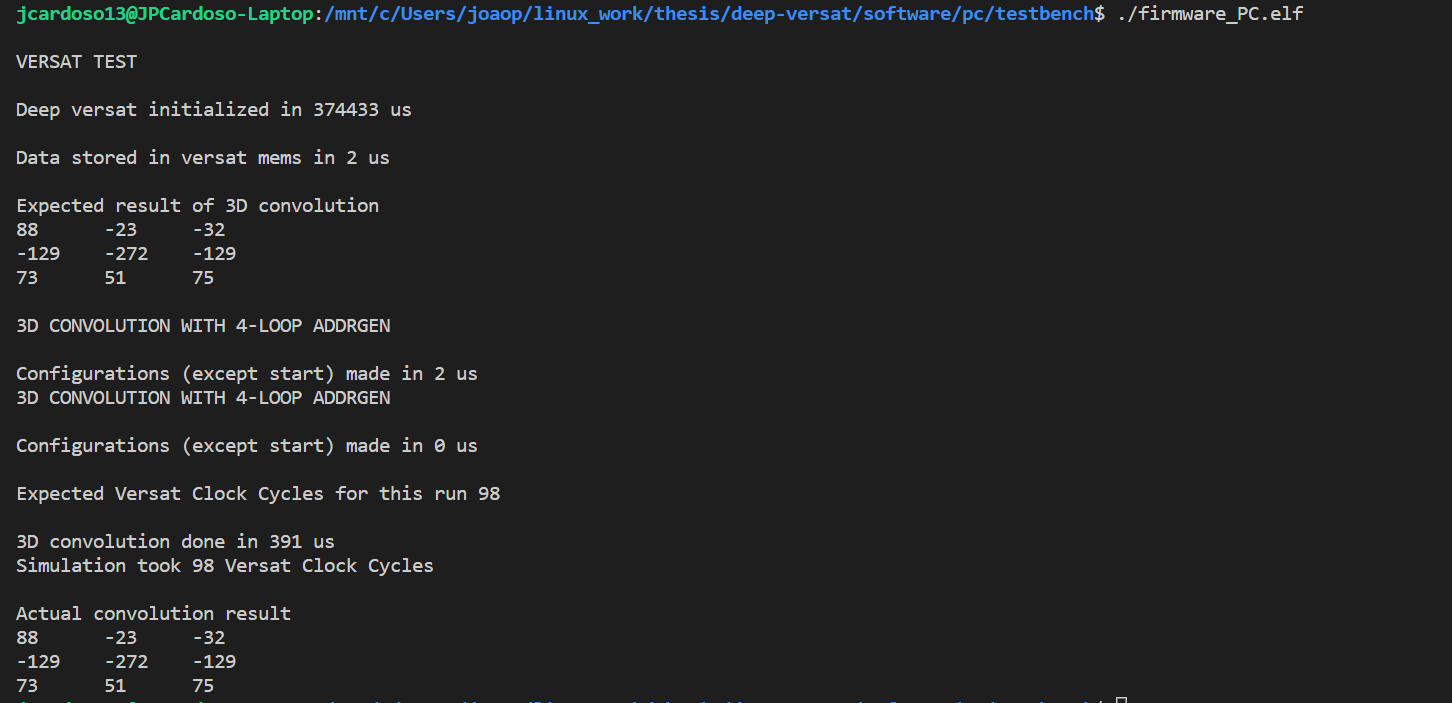
\includegraphics[width=\textwidth]{Figures/test1.png}
    \caption{Simulator test output in terminal}
    \label{figure:test1}
\end{figure} 

The estimated iterations needed are the following:

\[ Est=Delay+Iter_2*Per_2*Iter_1*Per_1\]

Where these are the AGU configurations of the VO where the results are written. The Delay is accumulated
through the several stages by adding two due to the MACs and ALUs.

%%%%%%%%%%%%%%%%%%%%%%%%%%%%%%%%%%%%%%%%%%%%%%%%%%%%%%%%%%%%%%%%%%%%%%%%
\section{Testing the new API}
\label{section:testgencov}

In this section, the same method for the previous testbench is made. 
While the previous one relies on using API v1 for the configuration, these test benches
run the new API. 

\subsection{Testbench for Matrix Multiplication}

The Matrix Multiplication is a quite simple program. The only thing needed is to an instance
Versat, run versat\_init(), create the matrixes, and then use the function matrix\_multiplication()
The data is also computed in the CPU the result to verify the output which can be found in
figure \ref{figure:test2}.

\begin{figure}[!htbp]
    \centering
    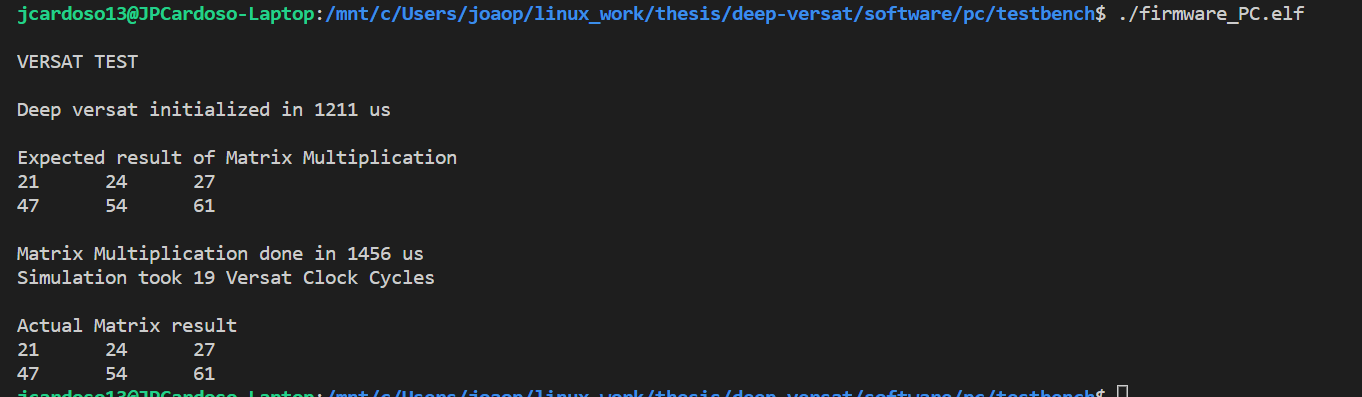
\includegraphics[width=\textwidth]{Figures/test2.png}
    \caption{Matrix Multiplication Testbench Outputs}
    \label{figure:test2}
\end{figure}

\subsection{Testbench for Generic Convolution}

Using the same method on the previous test benches, the following Convolution Layer was used
with several Versat Configurations.

\begin{table}[!htpb]
    \centering
    \begin{tabular}{ll}
    \hline
    \textbf{CNN Variable} & \textbf{Value}        \\ \hline
    Kernel Size            & 2                 \\
    Channels            & 2                       \\
    Number of Kernels            & 2                       \\
    Input Height                  & 12                        \\
    Input Width                & 12                  \\
    Stride              & 1                     \\
    Out Width               & 11                      \\
    Out Height            & 11  \\
    Out Channels                   & 2                     \\ \hline
    \end{tabular}
    \label{table:convInput}
    \caption{CNN Layer on the testbench}
\end{table}

With this layer, figure \ref{figure:test3} has the output result of the generic convolution testbench.
For this specific Versat hardware configuration the number of iterations needed is 711 using 3 Datapaths.

\begin{figure}[!htbp]
    \centering
    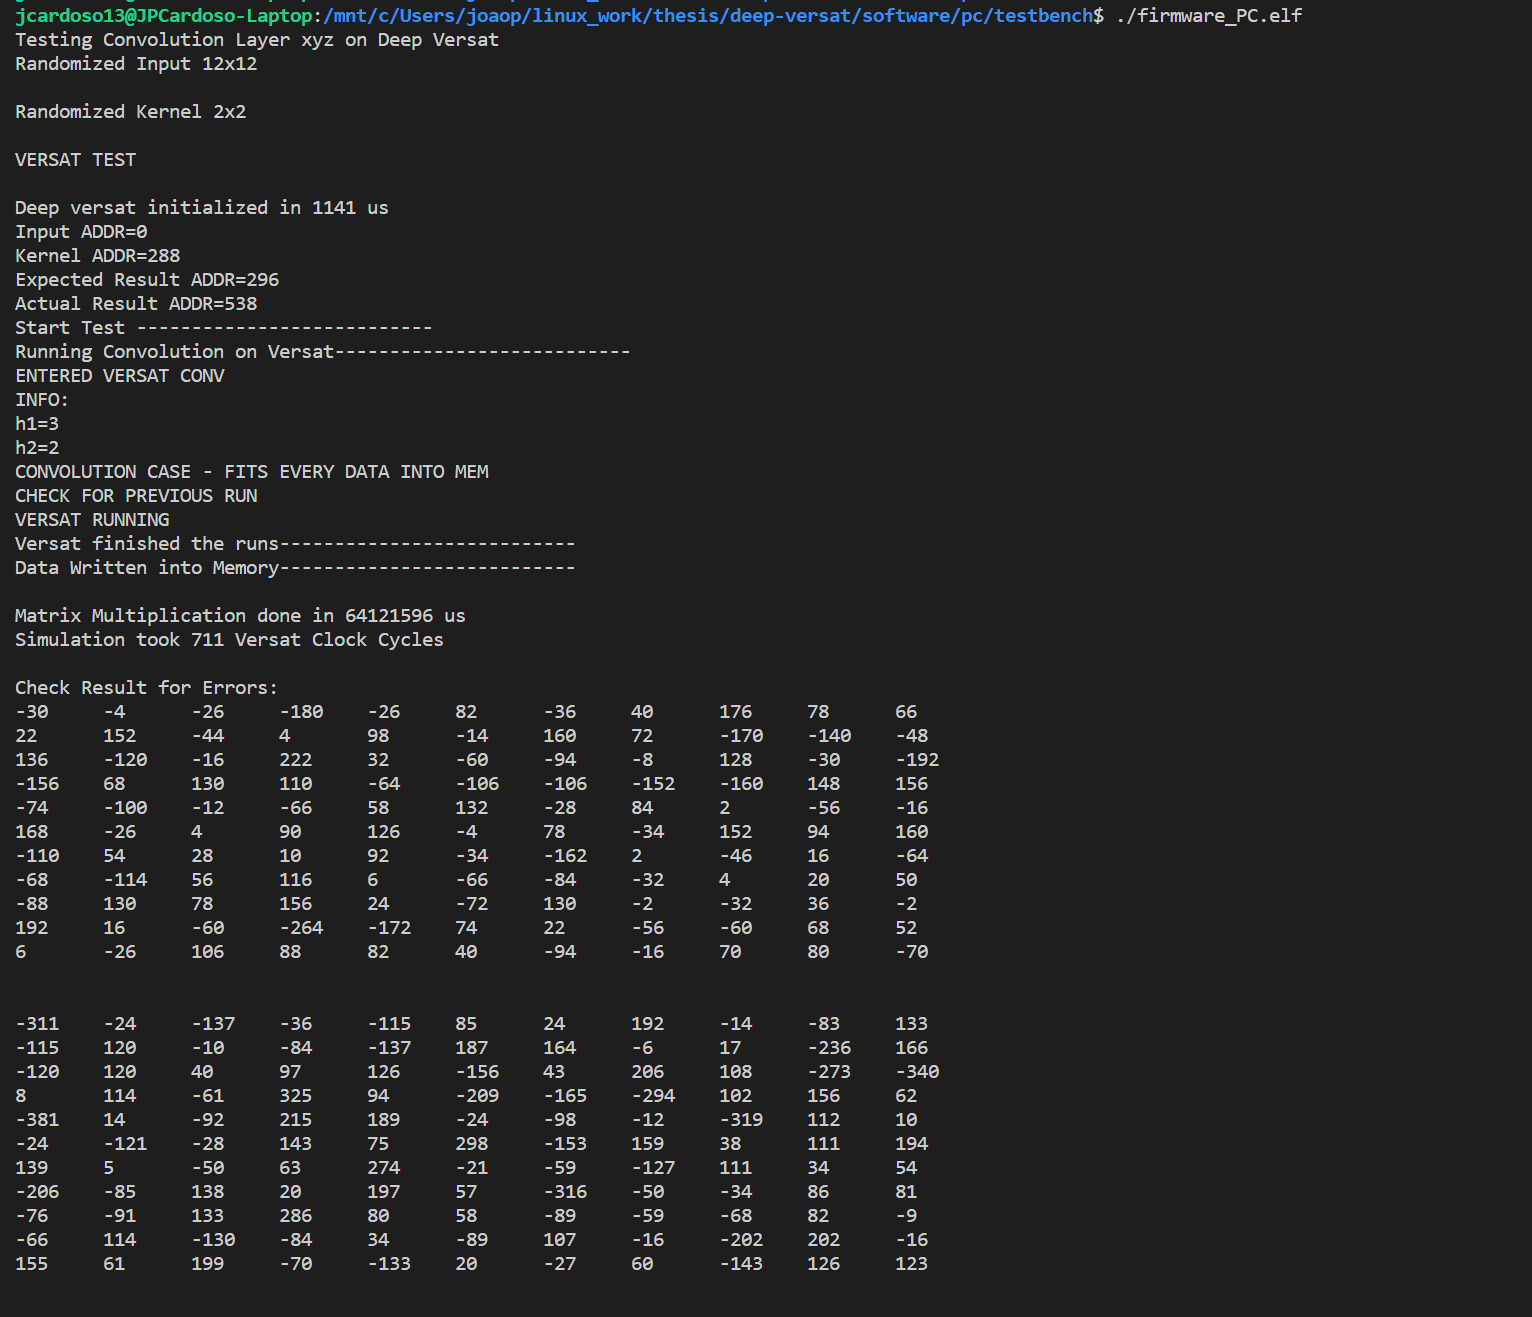
\includegraphics[width=\textwidth]{Figures/test3.png}
    \caption{Generic Convolution Testbench Outputs}
    \label{figure:test3}
\end{figure}

In Table \ref{table:Iterations}, the different Datapath numbers and how it affects performance.
A datapath is a combination of 1 VI, 1 MAC, and 1 VO. So the lower number in the Versat configuration file
decides the number of valid datapaths, of course, VI needs +1 in numbers more than the functional units due to the Kernel memory.
\newpage
\begin{table}[!htpb]
    \centering
    \begin{tabular}{ll}
    \hline
    \textbf{Number of Datapaths} &  \textbf{Iterations}        \\ \hline
    1          & 1943                 \\
	2          & 1063                 \\
	3          & 711                 \\
	4          & 535                 \\
	6          & 359                 \\
	8          & 359                 \\
	11          & 183                 \\
	16          & 183                 \\
    22            & 183                       \\  \hline
    \end{tabular}
    \label{table:Iterations}
    \caption{CNN Layer on the testbench with several Versat hardware configurations}
\end{table}

The reason for these results is quite simple. In total, 11 output lines are divided
by the datapaths. When the division is not a whole number, the remainder gets distributed
by available datapaths. The Consequence of this, when changing from 6 to 8 datapaths, the performance
doesn't get any better. Datapath 0 will have to run twice to (2 lines) while Datapath 8 will run 1 line.
To increase further the performance, the output channels would have to be divided through more datapaths.